%Input premable
\documentclass{beamer}

%Packages
\usepackage{graphicx}
\usepackage{graphics}
\usepackage{hyperref}
\usepackage[english]{babel}
\usepackage{amsmath}
\usepackage{amsfonts}
\usepackage{amssymb}
\usepackage{bm}
\usepackage{comment}
\usepackage{etoolbox}
\usepackage{graphicx}
\usepackage{tabularx,ragged2e,booktabs}
\usepackage{caption}
\usepackage{hyphenat}
\usepackage{fixltx2e}
\usepackage[para]{threeparttable}
\usepackage[capposition=top]{floatrow}
\usepackage{subcaption}
\usepackage{pdfpages}
\usepackage{natbib}
\usepackage{rotating}

%Math Functions
\DeclareMathOperator{\var}{Var}
\DeclareMathOperator{\cov}{Cov}

%Commands
\newcommand\independent{\protect\mathpalette{\protect\independenT}{\perp}}
\def\independenT#1#2{\mathrel{\rlap{$#1#2$}\mkern2mu{#1#2}}}
\newcommand{\overbar}[1]{\mkern 1.5mu\overline{\mkern-1.5mu#1\mkern-1.5mu}\mkern 1.5mu}
\newcommand{\equald}{\ensuremath{\overset{d}{=}}}

\newenvironment{wideitemize}{\itemize\addtolength{\itemsep}{10pt}}{\enditemize}

\mode<presentation>
	{
	\usetheme{UChicagoJorge}
	\setbeamercovered{transparent = 28}
	}

%\usecolortheme{UChicagoJorge} 
%\useinnertheme{UChicagoJorge}
%\useoutertheme{UChicagoJorge}

\title{College Enrollment and Dropout}
\subtitle{Stepping Stone and Option Value}
\author{Econ 350, Jorge L. Garc\'{i}a}
\date{This draft: \today}

\begin{document}


\begin{frame}[plain]
	\titlepage
\end{frame}


\AtBeginSection[]
{
   \begin{frame}
       \frametitle{Outline}
       \tableofcontents[currentsection]
   \end{frame}
}

\section{Ozdagli \& Trachter, 2011}

\begin{frame}
	\frametitle{Paper}
		\begin{itemize}
			\item On the Distribution of College Dropouts: Wealth and Uninsurable Idiosyncratic Risk
			\item 2011
			\item Ali K. Ozdagli (FRB-Boston) and Nicholas Trachter (FRB-Richmond)
			\item R\&R JOLE 
		\end{itemize}
\end{frame}

\begin{frame}
	\frametitle{Overview}
		\begin{itemize}
			\item Dynamic model of the decision to pursue college
				\begin{enumerate}
					\item Students' uncertainty: about future income stream due to unobserved scholastic ability
					\item Expectations reevaluation: on success in college after matriculation and after taking exams 
				\end{enumerate}
			\item Findings (only theoretical)
				\begin{enumerate}
					\item Poorer students are
						\begin{itemize}
							\item less likely to graduate
							\item likely to dropout sooner
						\end{itemize}
				\end{enumerate}
			\item Interesting feature: no need to introduce credit constraints
		\end{itemize}
\end{frame}

\begin{frame}
	\frametitle{Motivation}
		\begin{itemize}
			\item The authors motivate their work claiming that inequality perpetuates and exacerbates as follows in the U.S.:
				\begin{enumerate}
			\item Large fraction of every cohort that enrolls in colleges drops out
			\item High concentration of dropouts among students from lower-income families
			\item Students from low-income families drop out earlier than students from high-income families
			\item Less low-income individuals graduate from college
			\item High return to education
				\end{enumerate}
		\end{itemize}
\end{frame}

\begin{frame}
	\frametitle{Motivation, contd 1}
		\begin{figure}[H] 
		\caption*{}
		\centering
		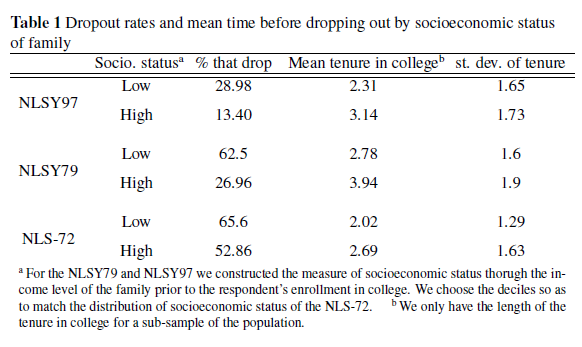
\includegraphics[width=3.5in, height=2in]{Figures/OT/table1.png}
		\end{figure}
\end{frame}

\begin{frame}
	\frametitle{Motivation, contd 2}
		\begin{figure}[H] 
		\caption*{}
		\centering
		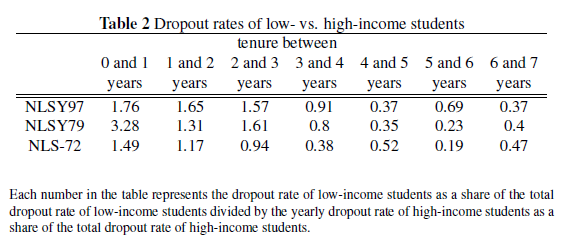
\includegraphics[width=3.5in, height=2in]{Figures/OT/table2.png}
		\end{figure}
\end{frame}

\begin{frame}
	\frametitle{Motivation, contd 3}
		\begin{figure}[H] 
		\caption*{}
		\centering
		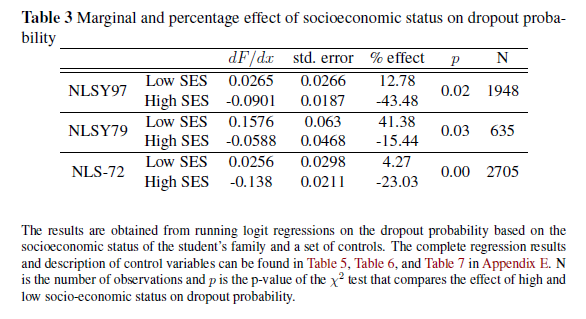
\includegraphics[width=3.5in, height=2in]{Figures/OT/table3.png}
		\end{figure}
\end{frame}

\begin{frame}
	\frametitle{Motivation, contd 4}
		\begin{figure}[H] 
		\caption*{}
		\centering
		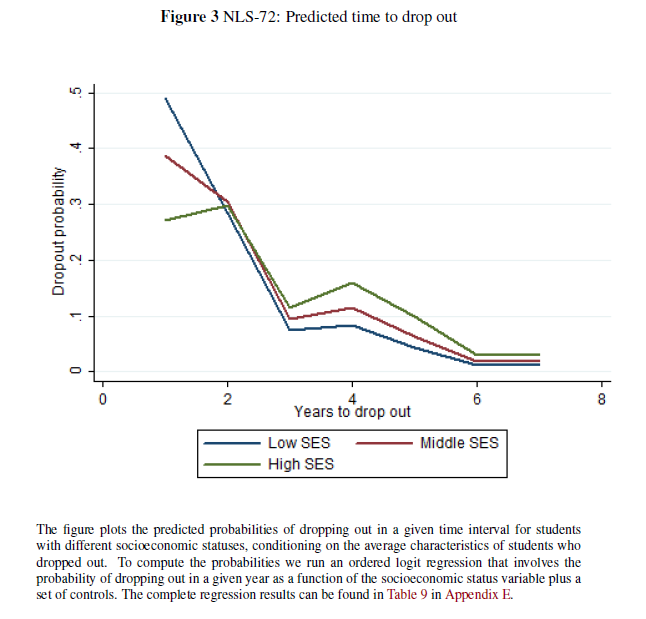
\includegraphics[width=2.5in, height=2.5in]{Figures/OT/figure3.png}
		\end{figure}
\end{frame}

\begin{frame}
	\frametitle{Motivation, contd 5}
		\begin{figure}[H] 
		\caption*{}
		\centering
		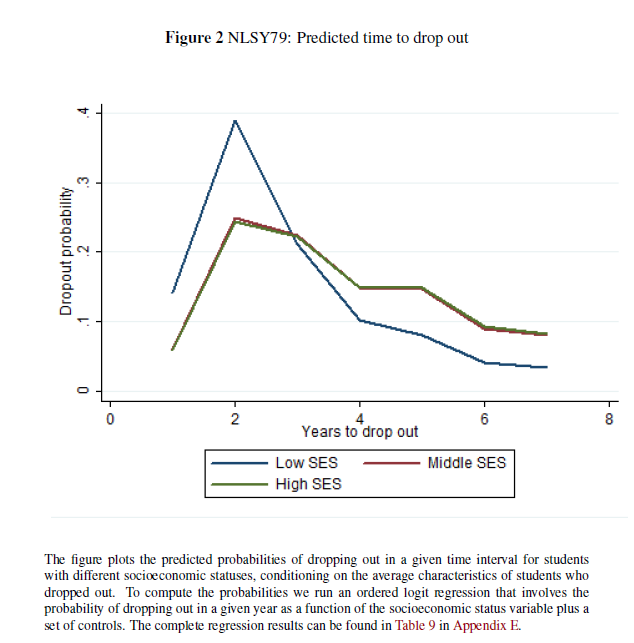
\includegraphics[width=2.5in, height=2.5in]{Figures/OT/figure2.png}
		\end{figure}
\end{frame}

\begin{frame}
	\frametitle{Motivation, contd 6}
		\begin{figure}[H] 
		\caption*{}
		\centering
		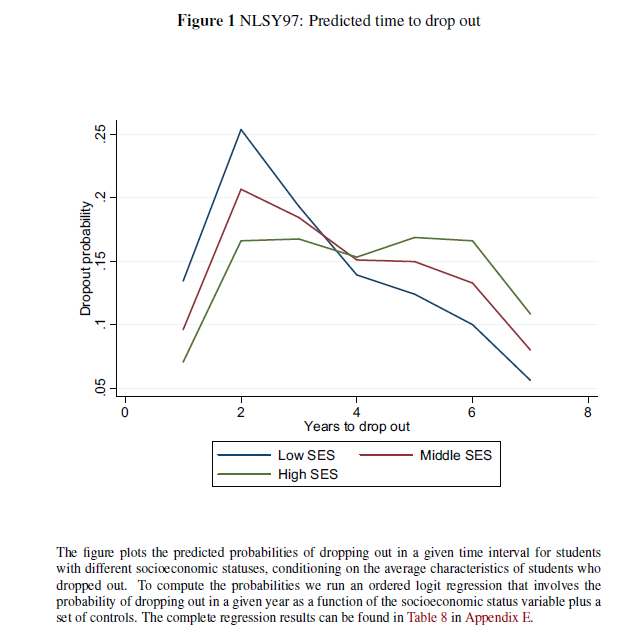
\includegraphics[width=2.5in, height=2.5in]{Figures/OT/figure1.png}
		\end{figure}
\end{frame}

\begin{frame}
	\frametitle{Model, Basics}
	\begin{itemize}
		\item Based on Miao and Wang (2007): framework of entrepreneurial learning and analysis
		\item Add relevant ingredients of dropout decision:
			\begin{enumerate}
				\item Wage profile: depends on experience and college graduation (and corresponding interaction)
				\item Include information unfolding through learning about unobserved ability in college
			\end{enumerate}
	\end{itemize}
\end{frame}

\begin{frame}
	\frametitle{Model, Information}
		\begin{itemize}
			\item The author argues that credit constraints and learning about risk are not fundamental
				\begin{itemize}
					\item Credit constrains: (i) $29\%$ of students from the richest families dropout (NLSY79); (ii) rising house prices lead to higher graduation rates, especially among low-income families (NLSY97)
					\item Learning about stochastic taste: no relation with wealth
				\end{itemize}
		\item Decides to model information unfolding through learning about ability
		\end{itemize}
\end{frame}

\begin{frame}
	\frametitle{Model, Primitives}
		\begin{itemize}
			\item Continuous time, finite horizon; $t \in [0,T]$
			\item At $t=0$
				\begin{enumerate}
					\item Initial endowment, $x(0) \equiv x_{0}$
					\item Unobserved ability to acquire human capital, $\mu \in \{0,1\}$
					\item Prior on ability, $\Pr(\mu = 1 | t = 0) = p(0) \equiv p_{0}$
					\item Either enrolled in college (full-time) or working (in low-skilled or high-skilled sector)
					\item High-skill sector only hires high-skilled workers with college degrees
				\end{enumerate}
			\item Work: absorbing state
			\item Wage function:
				\begin{eqnarray}
						\tilde{w} \left( \mu, \tau \right)
							\begin{cases}
								w(\tau) &,  \tau > 0 \\
								w_{0}    &,  \tau = 0, \mu = 0 \\
								w_{1}   &,  \tau = 0, \mu = 1 
							\end{cases} 
				\end{eqnarray}
\noindent with $\tau = T - t, w_{0} \equiv w(0) < w_{1}$; $\tau_{0} > \tau_{1} \Leftrightarrow w_{1} > w_{0}$. 
		\end{itemize}
\end{frame}

\begin{frame}
	\frametitle{Model, Primitives contd 1}
		\begin{figure}[H] 
		\caption*{Figure 4. Wage Function}
		\centering
		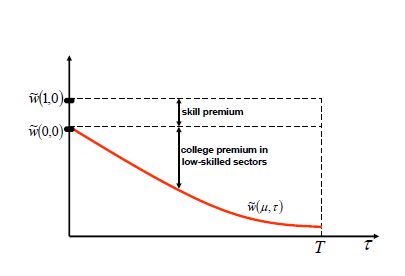
\includegraphics[width=2in, height=1.5in]{Figures/OT/figure4.png}
		\end{figure}
\end{frame}

\begin{frame}
	\frametitle{Model, Primitives contd 2}
		\begin{itemize}
			\item $c$, consumption
			\item $a$, per-unit of time cost of college
			\item $\rho$, discount rate; $r$, interest rate
			\item $\gamma$, CRRA parameter
			\item $\lambda_{1}$, probability of getting an excellent grade for high ability student
			\item $\lambda_{0}$, probability of getting a failing grade for low ability student
				\begin{itemize}
					\item Interpret $\lambda_{1},\lambda_{0}$ as speed of learning
					\item In a continuous (Brownian motion) setting this is analogue to having two volatility parameters
				\end{itemize}
		\end{itemize}
\end{frame}

\begin{frame}
	\frametitle{Model, Primitives contd 2}
		\begin{figure}[H] 
		\caption*{}
		\centering
		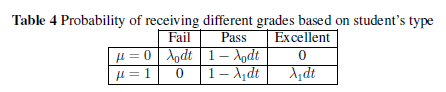
\includegraphics[width=2.5in, height=.5in]{Figures/OT/table4.png}
		\end{figure}
\end{frame}

\begin{frame}
	\frametitle{Model, Primitives contd 3}
		\begin{itemize}
			\item Evolution of wealth
				\begin{eqnarray}
					\dot{x} = 
						\begin{cases}
							rx + \tilde{w}(\mu, \tau) - c &, \text{if working} \\
							rx - a - c &, \text{if enrolled in college} \label{eq:x}
						\end{cases}
				\end{eqnarray}
		\end{itemize}
\end{frame}

\begin{frame}
	\frametitle{Model, Student's Problem (Sequential)}
		\begin{equation}
			\max _{ c(t)}\mathbb{E} \left\{ \int \limits _{0} ^{\infty} \exp ^{- \rho t} \frac{c(t)^{1 - \gamma}}{1 - \gamma} | p_{0}, x_{0}  \right\}
		\end{equation}
\noindent s.t. \eqref{eq:x} holds
\end{frame}

\begin{frame}
	\frametitle{Model, Student's Problem (Recursive)}
		\begin{itemize}
			\item $J(x,p,\tau)$, student's with current wealth $x$, prior on ability $p$, $\tau$ time before graduation value function
			\item $V(x,\mu,\tau)$, with current wealth $x$, type $\mu$, $\tau$ time before graduation value function
		\end{itemize}
\end{frame}

\begin{frame}
	\frametitle{Model, Worker's Value Function}
		\begin{itemize}
			\item Instantaneous utility derived: consumption + change in wealth
				\begin{equation}
					\rho V(x,\mu,\tau) = \max_{c} \frac{c^{1 - \gamma}}{1 - \gamma} + V_{x}(x,\mu,\tau)\dot{x}
				\end{equation}
			\item First order condition:
				\begin{equation}
					c^{- \gamma} = V_{x}(\cdot)
				\end{equation}
			\item Define $W(\mu, \tau)$ as the present value of earnings, let $A$ be a constant in terms of $\gamma, \rho$, and rearrange to get
				\begin{equation}
					V(x,\mu,\tau) = A \left( r \left[ x + W(\mu,\tau) \right]  \right)^{1 - \gamma} \label{eq:workers}
				\end{equation}
			\item Note that this implies that the fact that wages are constant is relatively easy to assume away by changing $W(\cdot)$ in \ref{eq:workers}
		\end{itemize}
\end{frame}

\begin{frame}
	\frametitle{Model, Student's Value Function with Known Types}
		\begin{itemize}
			\item Focus on $\mu = 1$ 
			\item For $\mu = 0$ we wait for the results (want to guarantee that $J(x,0,\tau) = V(x,0,\tau)$)
			\item Same principle leads to
				\begin{equation}
					\rho J(x,1,\tau) = \max_{c} \frac{c^{1-\gamma}}{1 - \gamma} + J_{x}(x,1,\tau) \dot{x} + J_{\tau}(x,1,\tau) \dot{\tau}  
				\end{equation}
\noindent with $J(x,1,0) = J(x,1,0)$
			\item First order condition
				\begin{equation}
					c^{1 - \gamma} = J(x,1,\tau) 
				\end{equation}
			\item Solve to get
				\begin{equation}
					J(x,1,\tau) = A \left[ r \left( x + \exp^{r \tau} W(1,0) - a \frac{1 - \exp^{r \tau}}{r} \right) \right]^{1 - \gamma}
				\end{equation}
		\end{itemize}
\end{frame}

\begin{frame}
	\frametitle{\begin{small} Student's Value Function with Unknown Types \end{small}}
	\begin{itemize}
		\item Difficulties
			\begin{enumerate}
				\item Wage upon graduation depends on true ability
				\item New information arrives after each exam
				\item Some students drop out
			\end{enumerate}
		\item Prior's evolution
			\begin{eqnarray}
				p(t+dt) =
					\begin{cases}
						0 &, \text{fails} \\
						1 &, \text{excellent grade} \\
						\frac{p(t) \left[1-\lambda_{1}dt \right]}{p(t) \left[1-\lambda_{1}dt \right] + (1-p(t)) \left[1-\lambda_{0}dt \right]} &, \text{otherwise}
					\end{cases}
			\end{eqnarray}
		\item If the student does not fail or has an excellent grade then
			\begin{equation}
				\dot{p} = - \left( \lambda_{1} - \lambda_{0} \right) p (1 - p)
			\end{equation}
	\end{itemize}		
\end{frame}

\begin{frame}
	\frametitle{Model, Time-line}
		\begin{figure}[H] 
		\caption*{}
		\centering
		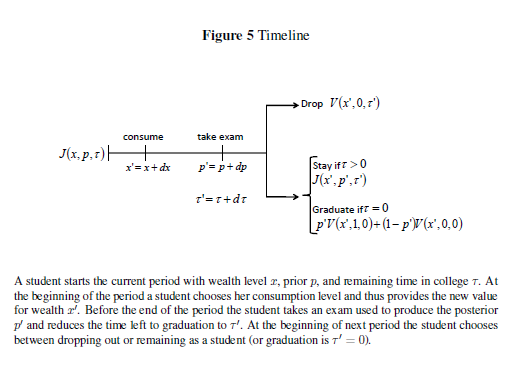
\includegraphics[width=2.5in, height=2in]{Figures/OT/figure5.png}
		\end{figure}
\end{frame}

\begin{frame}
	\frametitle{\begin{small} Student's Value Function with Unknown Types, contd 1 \end{small}}
		\begin{itemize}
			\item Same principle leads to		
			\begin{eqnarray}
				\rho J(x,p,\tau) &=& \max_{c} \frac{c^{1- \gamma}}{1- \gamma} + J_{x}(x,p,\tau)\dot{x} + J_{p}(x,p,\tau)\dot{p}  \nonumber \\ 
								 &+& J_{\tau}(x,p,\tau)\dot{\tau} + \lambda_{1} p \left[ J(x,1,\tau) - J(x,p,\tau) \right] \nonumber \\ 
								 &+& \lambda_{0} (1 - p) \left[ V(x,0,\tau) - J(x,p,\tau) \right] 
			\end{eqnarray}
			\item Define $p^*(x,\tau)$ as the threshold such that if $p \leq p^*(x,\tau)$ the student drops out college	
			\end{itemize}		
\end{frame}

\begin{frame}
	\frametitle{\begin{small} Student's Value Function with Unknown Types, contd 1 \end{small}}
		\begin{itemize}
			\item Terminal conditions
				\begin{enumerate}
					\item Terminal Condition
						\begin{equation}
							J(x,p,0) = p V(x,1,0) + (1-p) V(x,0,0) 
						\end{equation}
					\item Value Matching Condition
						\begin{equation}
							J(x,p^*(\cdot),\tau) = V(x,\tau,0)
						\end{equation}
					\item Smooth Pasting Conditions
						\begin{eqnarray}
							J_{p}(x,p^*(\cdot),\tau) &=& 0 \\
							J_{x}(x,p^*(\cdot),\tau) &=& V_{x}(x,\tau,0)\\
							J_{\tau}(x,p^*(\cdot),\tau) &=& V_{\tau}(x,\tau,0)
						\end{eqnarray}
				\end{enumerate}
		\end{itemize}
\end{frame}

\begin{frame}
	\frametitle{\begin{small} Student's Value Function with Unknown Types, contd 2 \end{small}}
		\begin{itemize}
			\item Use FOC to obtain
				\begin{equation}
					p^*(x,\tau) = \frac{a + rW(0,\tau) + W_{\tau} (0,\tau)}{\lambda_{1}} \frac{V_{x}(x,0,\tau)}{J(x,1,\tau) - V(x,0,\tau)}
				\end{equation}
		\end{itemize}
	
\end{frame}

\begin{frame}
	\frametitle{Results, Known Types}
		\begin{itemize}
			\item Lemma 1
				\begin{itemize}
					\item Assume $r \exp^{-r \tau} W(1,0) - a (1 - \exp^{-r \tau})  \geq r W(1, \tau)$
					\item A student of type $\mu = 1$ with current state $(x,\tau)$ chooses to remain in college until $\tau = 0$
					\item Intuition: graduation premium needs to be high enough for high-ability types to remain in college 
				\end{itemize}
			\item Lemma 2
				\begin{itemize}
					\item Assume $a + r W(0,\tau) + W_{\tau} (0,\tau) > 0$	
					\item A student of type $\mu = 0$ immediately drops college
					\item Intuition: if the per-unit marginal cost of attending college is positive, the low-skilled type student drops college immediately
					\item Implication: $J(x,0,\tau) = V(x,0,\tau)$
				\end{itemize}				 
		\end{itemize}
\end{frame}

\begin{frame}
	\frametitle{Results, Unknown Types}
		\begin{itemize}
			\item Result 1
				\begin{itemize}
					\item Let the assumptions in Lemmas 1 and 2 hold
					\item Students with a greater endowment have a lower value of $p^*$, i.e. the belief threshold for which they drop college is lower
					\begin{equation}
						\frac{\partial p^*(x, \tau)}{\partial x} < 0
					\end{equation}
				\end{itemize}
			\item Let $\tau^*$ denote the time to graduation at the moment individual joins the workforce
				\begin{itemize}
					\item $\tau^* = T$, joins workforce immediately
					\item $\tau^* = 0$, joins workforce with college degree
				\end{itemize}
		\end{itemize}
\end{frame}

\begin{frame}
	\frametitle{Results, Unknown Types contd 1}
		\begin{itemize}
			\item Proposition 1
				\begin{itemize}
					\item Consider two endowments $x_{0}^i, x_{0}^j$ with $x_{0}^i > x_{0}^j$
					\begin{equation}
					\forall \ \bar{\tau} \in \mathbb{R}_{++}, \Pr \{ \tau^* \leq \bar{\tau} | x_{0}^i, p_{0}, \mu \} = \Pr \{ \tau^* \leq \bar{\tau} | x_{0}^j, p_{0}, \mu \}
					\end{equation}
					\item Meaning: given a skill level. $\mu$, and a initial belief, $p_{0}$, richer students drop out later (and have longer expected tenures!)
					\item Intuition:
						\begin{itemize}
							\item Cannot diversify uncertainty related to the outcomes of college education
							\item College is riskier than the risk-free asset!
							\item CCRA: risk aversion is decreasing in wealth
							\item Students with more wealth invest more is riskier projects
						\end{itemize}
					\item Corollary: once condition on ability type and prior belief richer students are more likely to graduate from college
					\item Robust? Results hold for HARA utility iff the risk aversion parameter is decreasing in wealth
				\end{itemize}
		\end{itemize}
\end{frame}

\section{Trachter, 2014}

\begin{frame}
	\frametitle{Paper}
		\begin{itemize}
			\item Stepping Stone and Option Value in a Model of Post-Secondary Education
			\item 2014
			\item Nicholas Trachter (FRB-Richmond)
			\item R\&R QE
		\end{itemize}
\end{frame}

\begin{frame}
	\frametitle{Overview}
		\begin{itemize}
			\item Dynamic model of the student's  decision to switch from a 2-year (community) college to a 4-year college
			\begin{enumerate}
				\item Learn about uncertain educational outcomes
				\item Drop out or transfer to more rewarding schools
				\item Carry a fraction of the accumulated human capital
			\end{enumerate}
			\item Community college as a ``stepping stone'' which provides
				\begin{enumerate}
					\item Leaning
					\item Transferable human capital
				\end{enumerate}
			\item Analogous to Jovanovic and Nyarko (1997), workers move up in the work ladder once they acquire skills
			\item Main findings:
				\begin{enumerate}
					\item Option value (of transferring/dropping) explains a large part of the returns to school enrollment
					\item Enrollment in community college is driven by the option to ``transfer up''
					\item The value of the stepping stone itself is small
				\end{enumerate}
		\end{itemize}
\end{frame}

\begin{frame}
	\frametitle{Motivation}
		\begin{itemize}
			\item Based on facts of the NLS-72		
		\begin{figure}[H] 
			\caption*{}
			\centering
			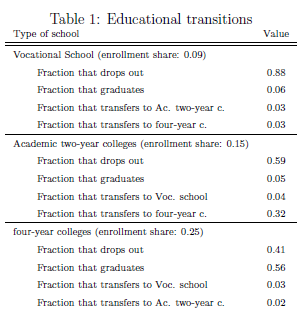
\includegraphics[width=1.5in, height=2in]{Figures/T/table1.png}
		\end{figure}
		
			\item Interesting fact: $56\%$ of students who transfer from community colleges to colleges graduate		
		\end{itemize}
\end{frame}

\begin{frame}
	\frametitle{Motivation, contd 1}
			\begin{figure}[H] 
				\caption*{}
				\centering
				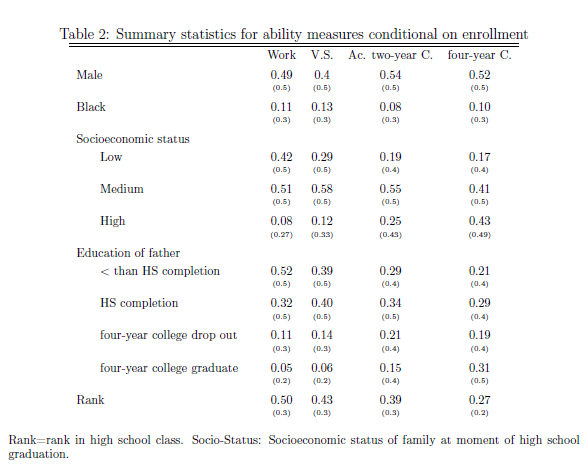
\includegraphics[width=2.5in, height=2.5in]{Figures/T/table2.png}
			\end{figure}
\end{frame}

\begin{frame}
	\frametitle{Motivation, contd 2}
		\begin{itemize}
			\item Why is community college a stepping stone?
				\begin{enumerate}
					\item Provides a less risky investment (than college) to learn about abilities
				\end{enumerate}
			\item Although empirically (almost) irrelevant, the model also allows for ``bandit steps''
				\begin{itemize}
					\item Enroll in the hardest step and move down the ladder
					\item Johnson (1978), Miller (1984)
				\end{itemize}
		\end{itemize}
\end{frame}

\begin{frame}
	\frametitle{Model, Primitives}
		\begin{itemize}
			\item Discrete time, infinite horizon; $t \in [0, \infty]$
			\item $\gamma$, CARA coefficient; $r$, interest/discount rate
			\item At $t=0$
				\begin{enumerate}
					\item Initial level of assets, $a_{0}$
					\item Unobserved ability to acquire human capital, $\mu \in \{0,1\}$
					\item Prior on ability, $\Pr(\mu = 1|t=0) = p(0) \equiv p_{0}$
				\end{enumerate}	
			\item The agent either
				\begin{enumerate}
					\item Works, $W$
					\item Four-year college, $C$
					\item Two-year college, $A$
				\end{enumerate}
			\item School credits, $s$
			\item Time before graduation tied to credit accumulation: $T^C > T^A$
			\item Evolution of credits tied to signals, $\eta \in \mathcal{H}$
			\item $\eta \sim f_{i}(\eta|\mu)$ for $i = A,C$ satisfies the MLRP
			\item Per-unit of time tuition: $\tau^C > \tau^A$
		\end{itemize}
\end{frame}

\begin{frame}
	\frametitle{Model, Primitives contd 1}
		\begin{itemize}
			\item Working: absorbing state
			\item Wage function:
				\begin{eqnarray}
					h(GS, i, \mu) = 
						\begin{cases}
							h^w &, GS = 0 \\
							h^i(\mu) &, GS =1
						\end{cases}
				\end{eqnarray}
\noindent with $GS = \mathbf{1}(\text{gradiation})$; $h^i (1) \geq h^i (0)$ for $i = C,A$ and $h^C(\mu) \geq h^A(\mu)$ for $\mu = 0,1$
			\item Evolution of assets
				\begin{eqnarray}
					a_{t+1} =
						\begin{cases}
							(1 + r)a_{t} + h(GS,i,\mu) - c_{t} &, \text{if working} \\
							(1+r)a_{t} - \tau^i - c_{t} &, \text{if enrolled in i}  \label{eq:a}
						\end{cases}
				\end{eqnarray}
				\item No borrowing constraints!
			\end{itemize}							
\end{frame}

\begin{frame}
	\frametitle{Model, Primitives contd 2}
		\begin{itemize}
			\item Evolution of credits
				\begin{equation}
					s' = s + \tilde{\Omega} (\eta, s)
				\end{equation}
\noindent with
				\begin{eqnarray}
					 \tilde{\Omega} (\eta, s) = 
					 	\begin{cases}
					 		\Omega(\eta) &, s < T^i \\
					 		0 &, s \geq T^i
					 	\end{cases}
				\end{eqnarray}
			\item Accumulation of credit is only a function of current signal
			\item Current signal has positive correlation with ability (MLRP)
			\item High-grade students accumulate at least as much credits as low-grade student: $\Omega(\eta_{1}) \geq \Omega(\eta_{2}) \Leftrightarrow \eta_{1} \geq \eta_{2}$
		\end{itemize}		 
\end{frame}

\begin{frame}
	\frametitle{Model, Primitives contd 3}
		\begin{itemize}
			\item Credits map \ldots for $i \neq j$ and $I = [A,C]$
				\begin{equation}
					\theta^i (s): \mathbb{R}_{+} \times I \rightarrow [0,T^j]
				\end{equation}
		\end{itemize}
\end{frame}

\begin{frame}
	\frametitle{Model, Student's Problem (Sequential)}
		\begin{itemize}
			\item Choose $c(t)$ and either to enroll, dropout, or transfer in $A,C$ to maximize
		\begin{equation}
			\mathbb{E} \left\{ \sum \limits _{t=0} ^{\infty}  \frac{\exp ^{- \gamma c_{t}} - 1}{- \gamma} | p_{0}, a_{0}  \right\}
		\end{equation}
\noindent s.t. \eqref{eq:a} holds
		\item CARA utility: order of risky projects is independent of financial wealth
		\end{itemize}
\end{frame}

\begin{frame}
	\frametitle{Model, Worker's Value Function}
		\begin{itemize}
			\item \ldots defined as
		\begin{equation}
			W(a;h) = max_{a',c} = \frac{\exp ^{- \gamma c_{t}} - 1}{- \gamma} + \frac{1}{1 + r} W(a';h)
		\end{equation}
\noindent with a' = (1 + r)a + h - c
			\item Use the FOC and solve to get
		\end{itemize}
			\begin{equation}
				W(a; h(GS, i, \mu)) = - \frac{1+r}{\gamma r} \exp^ {- \gamma (ra +  h(GS, i, \mu) )} + \frac{1+r}{\gamma r}			
			\end{equation}
\end{frame}

\begin{frame}
	\frametitle{Model, Beliefs and Governing CDF}
		\begin{itemize}
			\item Beliefs (use Baye's rule to obtain posterior)
				\begin{eqnarray}
					p ' &\equiv& b(\eta; p) \nonumber \\
						&=& \frac{1}{1 + \frac{f_{i}(\eta|\mu=0)}{f_{i}(\eta|\mu=1)} \frac{1-p}{p}}
				\end{eqnarray}
			\item Expected ``governing'' CDF
				\begin{equation}
					H_{i}(\eta, p) = p F_{i} (\eta | \mu = 1) + (1 - p) F_{i} (\eta | \mu = 0) 
				\end{equation}
		\end{itemize}
\end{frame}

\begin{frame}
	\frametitle{Model, Student's Value Function}
		\begin{itemize}
			\item \ldots defined as
				\begin{eqnarray}
				V_{i}(a,s,p) &=& \max_{a',c} \frac{\exp ^{- \gamma c_{t} -} - 1}{- \gamma} \nonumber \\  
				             &+& \frac{1}{1+r} \int \limits _{\eta \in \mathcal{H}} \tilde{V}_{i} (a',s',p') dH_{i}(\eta,p) \\
				 \tilde{V}_{i} (a',s',p') &=& \max \{ W(a'; h^w), \mathbf{1}(s' < T^i) V_{i}(a',s',p') \nonumber \\ 
				  &+& (1 - \mathbf{1}(s' < T^i)) p'W(a';h^i(1)) \nonumber \\       &+& (1 - \mathbf{1}(s' < T^i)) (1-p')W(a';h^i(0))   \nonumber \\      &,& V_{j}(a', \theta^i(s'),p')\}        
				\end{eqnarray}
\noindent with $i,j = A,C, i \neq j$
		\end{itemize}
\end{frame}

\begin{frame}
	\frametitle{Model, Timing}
		\begin{figure}[H] 
			\caption*{}
			\centering
			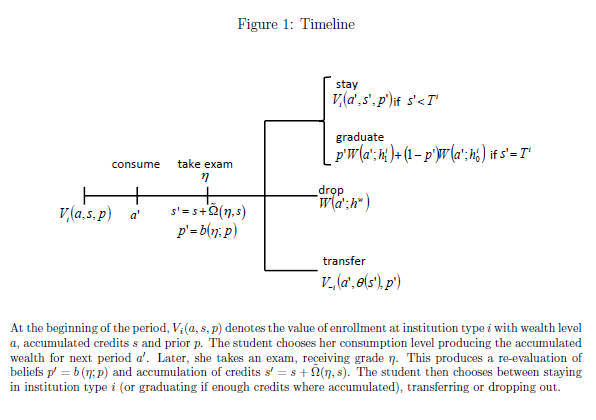
\includegraphics[width=3in, height=2.5in]{Figures/T/figure1.png}
		\end{figure}
\end{frame}

\begin{frame}
	\frametitle{Model, education pattern}
		\begin{itemize}
			\item Restrictions on
				\begin{itemize}
					\item Expected wages upon graduation
					\item Low-skill -high-skill wage differential
					\item Learning technology
					\item Tuition costs
				\end{itemize}
			\item \ldots enable to generate the desired pattern:
				\begin{itemize}
					\item Low ability individuals: better-off joining the workforce, if enrolled better-off in community college
					\item High ability individuals: better-off joining college, if not better-off in community college than in workforce
				\end{itemize}
			\item Community colleges are learning mechanism:
				\begin{enumerate}
					\item Pessimistic agents join the workforce
					\item Optimistic agents enroll in college
					\item Average join community colleges 
				\end{enumerate}
			\item ``A pessimist is a well informed optimist'' Mario Benedetti  			
		\end{itemize}
\end{frame}

\begin{frame}
	\frametitle{Calibration, Credits Map}
		\begin{itemize}
		\item Students who transfer from community colleges to colleges usually do so after the first year
		\item Students who transfer from colleges to community colleges spend for time studying after high school, on average
			\begin{eqnarray}
				\theta^i(s) =
				\begin{cases}
					\theta^i s ,& \theta^i s < T^j \\
					T^j        ,& \theta^i s \geq T^j
				\end{cases}
			\end{eqnarray}
\noindent with $\theta^A = \frac{1}{2}$ and $\theta^C = 0$
		\end{itemize}
\end{frame}

\begin{frame}
	\frametitle{Calibration, Signals and Credits}
		\begin{itemize}
		\item Signals are grades
			\begin{enumerate}
				\item Update beliefs
				\item Generate credit accumulation
				\item Fail(F), N(Neutral), Excel(E)
			\end{enumerate}
		\begin{eqnarray}
			\Omega(\eta) =
				\begin{cases}
					0 &, \eta = F \\
					1 &, \eta = N \\
					1 &, \eta = E
				\end{cases}
		\end{eqnarray}			
	\end{itemize}		
\end{frame}

\begin{frame}
	\frametitle{Calibration, Signals and Credits contd 1}
		\begin{itemize}
			\item $q_{\mu}^i(\eta)$: probability of each grade
				\begin{itemize}
					\item $q_{1}^A(F) = q_{0}^C(E) = 0$	
				\end{itemize}	
			\item Prior: estimate Ordered Probit on initial educational choice and construct
				\begin{eqnarray}
				p_{0} &=& \frac{1}{1 + \exp^{- X'\beta - \varepsilon}} \nonumber \\
				\varepsilon &\sim& \mathcal{N}(0,1) 
				\end{eqnarray}						 
		\end{itemize}
\end{frame}

\begin{frame}
	\frametitle{Calibration, Time Periods and Interest Rates}
		\begin{itemize}
		\item Time is measures in quarters: $T^A = 8, T^C = 16$
		\item Quarterly risk free interest rate $.45$
		\item $h^w$ is the numeraire (mean wage in 1985: \$17,740.63)
		\item $\tau^A = .1152$; $\tau^C = .3205$
		\item $\gamma = 8$; ($\gamma c = \sigma$)
		\end{itemize}
\end{frame}

\begin{frame}
	\frametitle{Calibration, the rest}
		\begin{itemize}
			\item Use Conditional Indirect Inference to calibrate the remaining parameters matching enrollment moments
				\begin{itemize}
					\item Long-run wage (4 parameters)
					\item Probability of dropout, transfer, and graduation (6 parameters)
					\item
				\end{itemize}
			\item Claims over-identification as follows: ``educational histories greatly differ across students in the sample and I have $3,462$, the model is over-identified''
			\item Calibration-Estimation satisfies MPLR and the structure necessary for the desired schooling pattern
			\item Transition probabilities implies by the model resemble the data
		\end{itemize}
\end{frame}

\begin{frame}
	\frametitle{Calibration-Estimation, Results}
			\begin{figure}[H] 
				\caption*{}
				\centering
				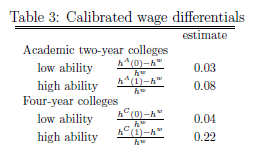
\includegraphics[width=2in, height=1.5in]{Figures/T/table3.png}
		\end{figure}
\end{frame}

\begin{frame}
	\frametitle{Calibration-Estimation, Results contd 1}
			\begin{figure}[H] 
				\caption*{}
				\centering
				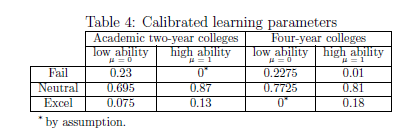
\includegraphics[width=3.5in, height=1in]{Figures/T/table4.png}
		\end{figure}
\end{frame}

\begin{frame}
	\frametitle{Calibration-Estimation, Fit}
			\begin{figure}[H] 
				\caption*{}
				\centering
				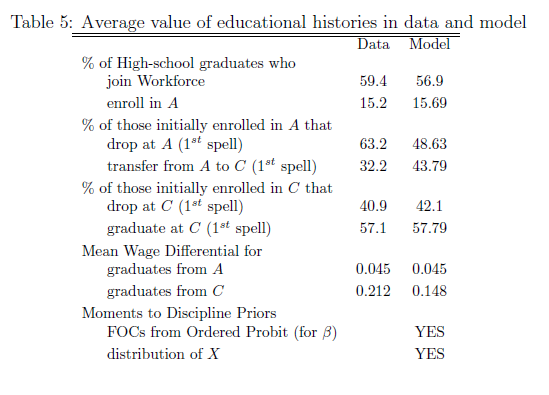
\includegraphics[width=2.5in, height=2in]{Figures/T/table5.png}
		\end{figure}
\end{frame}

\begin{frame}
	\frametitle{Calibration-Estimation, Fit}
			\begin{figure}[H] 
				\caption*{}
				\centering
				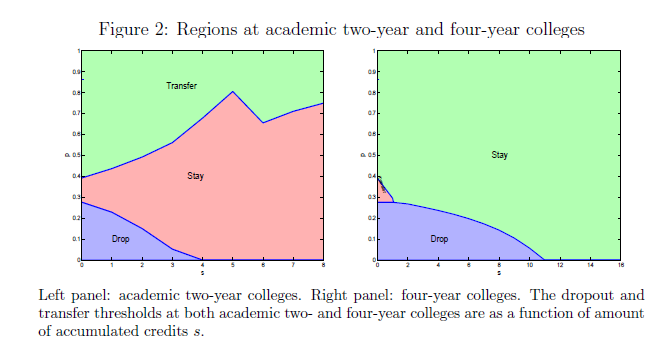
\includegraphics[width=3.5in, height=2in]{Figures/T/figure2.png}
			\end{figure}
\end{frame}

\begin{frame}
		\frametitle{Counter-factual Analysis}
		\begin{itemize}
			\item Compute the value of
				\begin{enumerate}
					\item Let $\gamma \rightarrow 0$ (risk neutrality)
					\item Rule out transfer option
					\item Rule out transfer and dropout options 
				\end{enumerate}
			\item Compute the value added of each component through decomposition of enrollment returns, $R_{i}(p)$
				\begin{eqnarray}
					R_{i}(p) &=& \frac{\Delta_{i}(p)}{\frac{1+r}{r}h^w} \nonumber \\
					W(a; h^w)&=& V_{i}(a - \Delta_{i}(p), 0, p)
				\end{eqnarray}
		\end{itemize}
\end{frame}

\begin{frame}
	\frametitle{Counter-factual Analysis, Return Decomposition}
		\begin{itemize}
			\item Decompose return as value added from: transfer option + dropout option + enrollment
			\begin{eqnarray}
			R_{i}^{E+D+T} &=& (R_{i}^{E+D+T} - R_{i}^{E+D}) \nonumber \\
			              &+& (R_{i}^{E+D} - R_{i}^{E}) + R_{i}^{E}
			\end{eqnarray}
		\end{itemize}
\end{frame}

\begin{frame}
	\frametitle{Counter-factual Analysis, Results}
		\begin{figure}[H] 
				\caption*{}
				\centering
				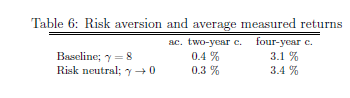
\includegraphics[width=3in, height=1in]{Figures/T/table6.png}
		\end{figure}
\end{frame}

\begin{frame}
	\frametitle{Counter-factual Analysis, Results contd 1}
		\begin{figure}[H] 
				\caption*{}
				\centering
				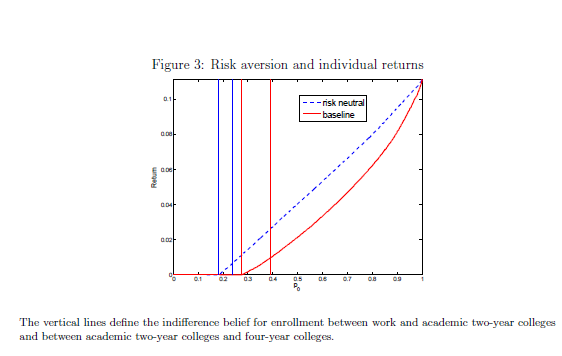
\includegraphics[width=2.3in, height=2in]{Figures/T/figure3.png}
		\end{figure}
\end{frame}

\begin{frame}
	\frametitle{Counter-factual Analysis, Results contd 2}
		\begin{figure}[H] 
				\caption*{}
				\centering
				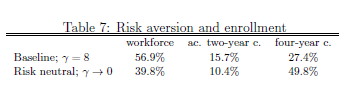
\includegraphics[width=3in, height=1in]{Figures/T/table7.png}
		\end{figure}
\end{frame}

\begin{frame}
	\frametitle{Counter-factual Analysis, Results contd 1}
		\begin{figure}[H] 
				\caption*{}
				\centering
				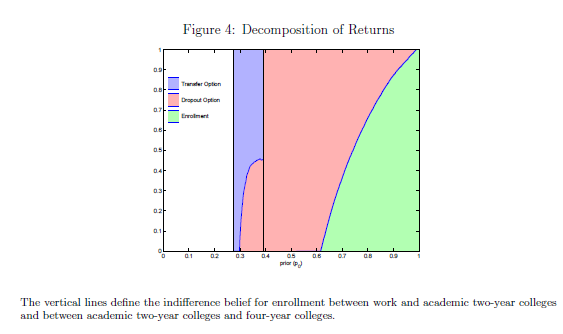
\includegraphics[width=2.3in, height=2in]{Figures/T/figure4.png}
		\end{figure}
\end{frame}

\begin{frame}
	\frametitle{Counter-factual Analysis, Results contd 2}
		\begin{figure}[H] 
				\caption*{}
				\centering
				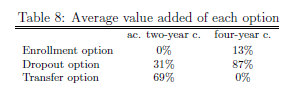
\includegraphics[width=3in, height=1in]{Figures/T/table8.png}
		\end{figure}
\end{frame}




























\end{document}